Il periodo di verifica e validazione inizia con la consegna della RQ e termina con la consegna della RA.\newline
Durante questo periodo, sono svolte le seguenti attività:
\begin{itemize}
	\item \textbf{Incremento: }modifiche incrementali ai seguenti documenti, ove necessario:
	\begin{itemize}
		\item Analisi dei requisiti;
		\item Piano di progetto;
		\item Piano di qualifica;
		\item Glossario;
		\item Norme di progetto;
		\item Specifica Tecnica;
		\item Definizione di Prodotto;
		\item Manuale Utente;
	\end{itemize}
	\item \textbf{Validazione e collaudo: }il prodotto viene testato per accertarsi che soddisfi tutti i requisiti prestabiliti.
\end{itemize}


\begin{figure}[H]
	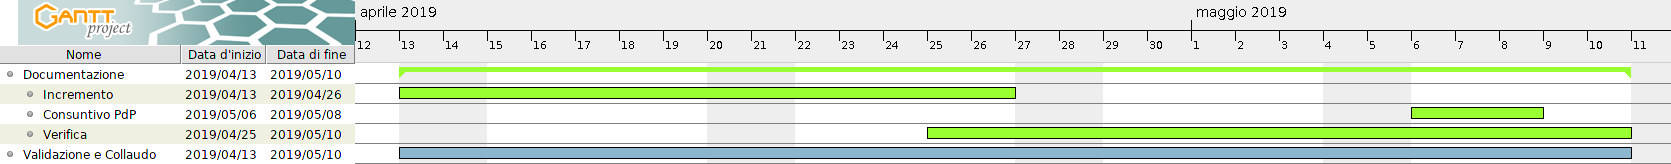
\includegraphics[width=1\linewidth]{Pianificazione/Verifica_Validazione.png}
	\caption{Diagramma di Gantt del periodo di verifica e validazione}
\end{figure}